\section{二重积分}
	\subsection{概念与性质}

	\begin{ti}
		计算 $\iint_{D} \bigl( x^{2} + y^{2} \bigr)^{\frac{3}{2}} \dd{\sigma}$,其中 $D = \bigl\{ (x,y) \bigl| x^{2} + y^{2} \leq 1, x^{2} + y^{2} \leq 2x \bigr\}$.
	\end{ti}

	\begin{ti}
		计算 $\iint_{D} \sqrt{x^{2} + y^{2}} \dd{x} \dd{y}$,其中 $D = \bigl\{ (x,y) \bigl| 0 \leq x \leq 1, 0 \leq y \leq 1 \bigr\}$.
	\end{ti}

	\begin{ti}
		计算
		\[
			I = \iint_{D} \frac{1 + y + y \ln \bigl( x + \sqrt{1 + x^{2}} \bigr)}{1 + x^{2} + y^{2}} \dd{\sigma},
		\]
		其中 $D = \bigl\{ (x,y) \bigl| x^{2} + y^{2} \leq 1, x \geq 0 \bigr\}$.
	\end{ti}

	\begin{ti}
		设 $f(x)$ 为连续的奇函数,平面区域 $D$ 由 $y = -x^{3}$,$x = 1$ 与 $y = 1$ 围成,计算 $I = \iint_{D} \bigl[ x^{2} + f(xy) \bigr] \dd{\sigma}$.
	\end{ti}

	\begin{ti}
		若 $D$ 是由直线 $x = -2$,$y = 0$,$y = 2$ 以及曲线 $x = -\sqrt{2y - y^{2}}$ 所围成的平面区域,计算 $I = \iint_{D} y \dd{x} \dd{y}$.
	\end{ti}

	\begin{ti}
		若 $D$ 是由圆 $x^{2} + y^{2} = 4$ 与 $(x + 1)^{2} + y^{2} = 1$ 所围成的平面区域(如图~\ref{fig:1.5.1}),计算 $I = \iint_{D} \bigl( \sqrt{x^{2} + y^{2}} + y \bigr) \dd{\sigma}$.
		\begin{figure}[htbp]
			\centering
			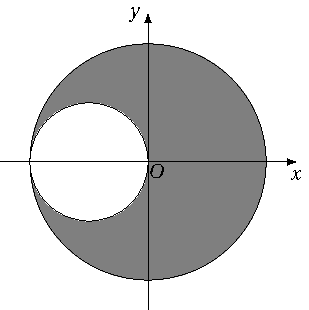
\includegraphics[scale=1]{figure/fig1-5-1.pdf}
			\caption{}\label{fig:1.5.1}
		\end{figure}
	\end{ti}

	\begin{ti}
		设 $D = \bigl\{ (x,y) \bigl| x^{2} + y^{2} \leq 1 \text{\ 且\ } x + y \geq 0 \bigr\}$,$f$ 为连续函数,计算
		\[
			I = \iint_{D} xy \bigl[ x + f\bigl( x^{2} - y^{2} \bigr) \bigr] \dd{x} \dd{y}.
		\]
	\end{ti}

	\begin{ti}
		设 $I(a) = \iint_{D} (x + y) \dd{x} \dd{y}$,其中 $D$ 由直线 $x = a$,$x = 0$,$y = a$,$y = -a$ 及曲线 $x^{2} + y^{2} = ax(a > 0)$ 所围成,计算 $I(a)$.
	\end{ti}

	\begin{ti}
		$\int_{-1}^{1} \dd{x} \int_{|x|}^{\sqrt{2 - x^{2}}} \sin \bigl( x^{2} + y^{2} \bigr) \dd{y} = $\kuo.

		\twoch{$\frac{\uppi}{4}(\cos 2 - 1)$}{$\frac{\uppi}{4}(- \cos 2 + 1)$}{$\frac{\uppi}{4}(\cos 2 + 1)$}{$\frac{\uppi}{4}(- \cos 2 - 1)$}
	\end{ti}

	\begin{ti}
		设平面区域 $D$ 由曲线 $y = \sin x \bigl( - \frac{\uppi}{2} \leq x \leq \frac{\uppi}{2} \bigr)$,$x = -\frac{\uppi}{2}$,$y = 1$ 围成,则 $\iint_{D} \bigl( xy^{3} - 1 \bigr) \dd{\sigma}$ 等于\kuo.

		\fourch{$2$}{$-2$}{$\uppi$}{$-\uppi$}
	\end{ti}

	\begin{ti}
		记平面区域 $D = \bigl\{ (x,y) \bigl| |x| + |y| \leq 1 \bigr\}$,计算如下二重积分:
		\begin{enumerate}
			\item $I_{1} = \iint_{D} \frac{af(x) + bf(y)}{f(x) + f(y)} \dd{\sigma}$,其中 $f(t)$ 为定义在 $(-\infty,$ $+\infty)$ 内的连续正值函数,常数 $a > 0, b > 0$;
			\item $I_{2} = \iint_{D} \bigl( \ee^{\lambda x} - \ee^{-\lambda y} \bigr) \dd{\sigma}$,常数 $\lambda > 0$.
		\end{enumerate}
	\end{ti}

	\begin{ti}
		设 $p(x)$ 在 $[a,b]$ 上非负且连续,$f(x)$ 与 $g(x)$ 在 $[a,b]$ 上连续且有相同的单调性,其中
		\[
			D = \bigl\{ (x,y) \bigl| a \leq x \leq b, a \leq y \leq b \bigr\},
		\]
		比较
		\begin{align*}
			I_{1} &= \iint_{D} p(x) f(x) p(y) g(y) \dd{x} \dd{y},\\
			I_{2} &= \iint_{D} p(x) f(y) p(y) g(y) \dd{x} \dd{y}
		\end{align*}
		的大小,并说明理由.
	\end{ti}